% Template for PLoS
% Version 3.1 February 2015
%
% To compile to pdf, run:
% latex plos.template
% bibtex plos.template
% latex plos.template
% latex plos.template
% dvipdf plos.template
%
% % % % % % % % % % % % % % % % % % % % % %
%
% -- IMPORTANT NOTE
%
% This template contains comments intended
% to minimize problems and delays during our production
% process. Please follow the template instructions
% whenever possible.
%
% % % % % % % % % % % % % % % % % % % % % % %
%
% Once your paper is accepted for publication,
% PLEASE REMOVE ALL TRACKED CHANGES in this file and leave only
% the final text of your manuscript.
%
% There are no restrictions on package use within the LaTeX files except that
% no packages listed in the template may be deleted.
%
% Please do not include colors or graphics in the text.
%
% Please do not create a heading level below \subsection. For 3rd level
% headings, use \paragraph{}.
%
% % % % % % % % % % % % % % % % % % % % % % %
%
% -- FIGURES AND TABLES
%
% Please include tables/figure captions directly after the paragraph where they
% are first cited in the text.
%
% DO NOT INCLUDE GRAPHICS IN YOUR MANUSCRIPT
% - Figures should be uploaded separately from your manuscript file.
% - Figures generated using LaTeX should be extracted and removed from the PDF
% before submission.
% - Figures containing multiple panels/subfigures must be combined into one
% image file before submission.
% For figure citations, please use "Fig." instead of "Figure".
% See http://www.plosone.org/static/figureGuidelines for PLOS figure guidelines.
%
% Tables should be cell-based and may not contain:
% - tabs/spacing/line breaks within cells to alter layout or alignment
% - vertically-merged cells (no tabular environments within tabular
% environments, do not use \multirow)
% - colors, shading, or graphic objects
% See http://www.plosone.org/static/figureGuidelines#tables for table
% guidelines.
%
% For tables that exceed the width of the text column, use the adjustwidth
% environment as illustrated in the example table in text below.
%
% % % % % % % % % % % % % % % % % % % % % % % %
%
% -- EQUATIONS, MATH SYMBOLS, SUBSCRIPTS, AND SUPERSCRIPTS
%
% IMPORTANT
% Below are a few tips to help format your equations and other special
% characters according to our specifications. For more tips to help reduce the
% possibility of formatting errors during conversion, please see our LaTeX
% guidelines at http://www.plosone.org/static/latexGuidelines
%
% Please be sure to include all portions of an equation in the math environment.
%
% Do not include text that is not math in the math environment. For example, CO2
% will be CO\textsubscript{2}.
%
% Please add line breaks to long display equations when possible in order to fit
% size of the column.
%
% For inline equations, please do not include punctuation (commas, etc) within
% the math environment unless this is part of the equation.
%
% % % % % % % % % % % % % % % % % % % % % % % %
%
% Please contact latex@plos.org with any questions.
%
% % % % % % % % % % % % % % % % % % % % % % % %

\documentclass[10pt,letterpaper]{article}
\usepackage[top=0.85in,left=2.75in,footskip=0.75in]{geometry}

% Use adjustwidth environment to exceed column width (see example table in text)
\usepackage{changepage}

% Use Unicode characters when possible
\usepackage[utf8]{inputenc}

% textcomp package and marvosym package for additional characters
\usepackage{textcomp,marvosym}

% fixltx2e package for \textsubscript
\usepackage{fixltx2e}

% amsmath and amssymb packages, useful for mathematical formulas and symbols
\usepackage{amsmath,amssymb}

% cite package, to clean up citations in the main text. Do not remove.
\usepackage{cite}

% Use nameref to cite supporting information files (see Supporting Information
% section for more info)
\usepackage{nameref}
\usepackage[colorlinks=true,linkcolor=blue,citecolor=blue,urlcolor=blue]{hyperref}

% line numbers
\usepackage[right]{lineno}

% ligatures disabled
\usepackage{microtype}
\DisableLigatures[f]{encoding = *, family = * }

% rotating package for sideways tables
\usepackage{rotating}

% Remove comment for double spacing
%\usepackage{setspace}
%\doublespacing

% Text layout
\raggedright
\setlength{\parindent}{0.5cm}
\textwidth 5.25in
\textheight 8.75in

% Bold the 'Figure #' in the caption and separate it from the title/caption with
% a period
% Captions will be left justified
\usepackage[aboveskip=1pt,labelfont=bf,labelsep=period,justification=raggedright,
singlelinecheck=off]{caption}

% Use the PLoS provided BiBTeX style
\bibliographystyle{plos2015}

% Remove brackets from numbering in List of References
\makeatletter
\renewcommand{\@biblabel}[1]{\quad#1.}
\makeatother

% Leave date blank
\date{}

% Header and Footer with logo
\usepackage{lastpage,fancyhdr,graphicx}
\usepackage{epstopdf}
\pagestyle{myheadings}
\pagestyle{fancy}
\fancyhf{}
\lhead{\includegraphics[width=2.0in]{PLOS-submission.eps}}
\rfoot{\thepage/\pageref{LastPage}}
\renewcommand{\footrule}{\hrule height 2pt \vspace{2mm}}
\fancyheadoffset[L]{2.25in}
\fancyfootoffset[L]{2.25in}
\lfoot{\sf PLOS}

% To-do notes
\usepackage{todonotes}

%% Include all macros below

\newcommand{\lorem}{{\bf LOREM}}
\newcommand{\ipsum}{{\bf IPSUM}}

%% END MACROS SECTION


\begin{document}
\linenumbers
\vspace*{0.35in}

% Title must be 250 characters or less.
% Please capitalize all terms in the title except conjunctions, prepositions,
% and articles.
\begin{flushleft}

{\Large \textbf\newline{Measurements on a 1:6 scale DOE Reference Model 2
cross-flow hydrokinetic turbine at transitional Reynolds numbers: Power production,
near-wake dynamics, and blade support strut losses}}
\newline
% Insert author names, affiliations and corresponding author email (do not include
% titles, positions, or degrees).
\\
Peter Bachant\textsuperscript{1,*},
Martin Wosnik\textsuperscript{1},
Budi Gunawan\textsuperscript{2},
Vincent Neary\textsuperscript{2}
\\
\bigskip
\bf{1} Center for Ocean Renewable Energy, University of New Hampshire, Durham, NH,
USA
\\
\bf{2} Water Power Technologies, Sandia National Laboratories, Albuquerque, NM, USA
\\
\bigskip

% Use the asterisk to denote corresponding authorship and provide email address
% in note below.
* pxL3@unh.edu

\end{flushleft}

% Please keep the abstract below 300 words
\section*{Abstract}

The mechanical power, total rotor drag, and near-wake flow of a 1:6 scale
Reference Model 2 (RM2) vertical-axis cross-flow turbine were measured in a
towing tank. Performance was measured at multiple Reynolds numbers by varying
tow carriage speed, and weak linear $Re$-dependence was achieved at a turbine
diameter Reynolds number $Re_D \approx 10^6$. An optimal tip speed ratio
$\lambda_0 = 3.1$ was chosen, at which the near wake velocity was measured at 1
m $(x/D=0.93)$ downstream. Mean velocity, turbulence, and mean kinetic energy
transport mechanisms were compared and contrasted with results from a high
solidity turbine acquired with the same test apparatus. Overall, lower levels of
streamwise wake recovery were calculated for the RM2 rotor---a consequence of
both the relatively low solidity and tapered blades. The effects of blade
support strut drag on turbine performance were investigated by covering the
rotor's NACA 0021 struts with cylinders. As expected, this modification
drastically reduced rotor power coefficient. Strut drag was also measured for
the NACA 0021 and cylindrical configurations with the blades removed. These
measurements provide a comprehensive open dataset for validating numerical
models' predictive capabilities for low solidity rotors.


\section*{Introduction}

Sandia National Laboratories, in collaboration with the US Department of Energy
developed the Reference Model devices to provide modeling targets for advancing
marine hydrokinetic (MHK) energy technology \cite{Neary2014}. The Reference
Model 2 (RM2), a vertical-axis cross-flow turbine intended for river
environments, was initially designed by Barone et al. \cite{Barone2011} using
the CACTUS vortex line code \cite{Murray2011}. A scaled physical model of the
RM2 was then designed and built by the Saint Anthony Falls Laboratory (SAFL) to
validate the CACTUS predictions. Experimental performance measurements were
significantly lower than the numerical results \cite{Hill2014}, which was
assumed to be a result of the physical model's low Reynolds number
\begin{equation}
    Re_D = \frac{U_\infty D}{\nu},
\label{eq:Re}
\end{equation}
where $U_\infty$ is the free stream velocity, $D$ is the rotor diameter (note
that in some cases the blade chord length $c$ is used as this length scale), and
$\nu$ is the fluid kinematic viscosity.

As a consequence of the inherently unsteady nature of the cross-flow rotor, the
RM2 blades experience large variations in angles of attack as they rotate about
their axis (``cross-flow'' means the axis of rotation is perpendicular to flow
direction). These variations become larger at lower tip speed ratio
\begin{equation}
    \lambda=\frac{\omega R}{U_\infty},
\end{equation}
where $\omega$ and $R$ are the rotor angular velocity and radius
\cite{Para2002}. Typically, the maximum angles of attack are sufficiently large
that the blades operate under dynamic stall, which is a complex unsteady process
and deviates significantly from static foil behavior, during part of the
rotation. Furthermore, the higher the solidity of a cross-flow turbine, the
lower the optimal tip-speed ratio at which it operates. Marine Hydrokinetic
(MHK) cross-flow turbines typically have higher solidity than cross-flow wind
turbines (VAWT), and hence operate at lower tip-speed ratios. Since MHK turbines
operate in a higher density fluid, unsteady dynamic effects related to the
blades' pitching motion and flow curvature also become more important when
compared to wind turbines.

The performance of cross-flow MHK turbines thus depends on both Reynolds number
and solidity (note that these issues are related, since an average blade chord
Reynolds number, $Re_{c,\mathrm{avg}} \approx \lambda U_\infty c/ \nu$, can be
expressed in terms of tip speed ratio $\lambda$, the optimal value of which is a
function of solidity). If numerical models are validated with physical model
data that was obtained at insufficiently high Reynolds numbers, it cannot be
determined whether problems with model predictions are caused by Reynolds number
effects, issues related to higher solidity, or both. It is uncertain whether
numerical models validated with physical model data obtained at low Reynolds
number should be considered validated at all, since the scale at which the model
will be applied is orders of magnitude larger. One way to overcome this
uncertainty is to show that the scaled physical model test has become Reynolds
number independent, and therefore validation efforts should be relevant at
full-scale.

For example, the effect of Reynolds number on average power output was shown to
be significant on the 2 m Sandia Research Darrieus turbine in wind tunnel
testing \cite{Blackwell1976}: Maximum power coefficient, $C_{P_{\max}}$,
increased with Reynolds number, $Re_c$, along with a shift of the location of
$C_{P_{\max}}$ toward lower tip speed ratios due to delayed blade stall. The
effects of Reynolds number were quite dramatic over a relatively small range of
$Re_c \approx 1.1 \times 10^5$--$2.9 \times 10^5$. More recently, Bachant and
Wosnik \cite{Bachant2014, Bachant2015-RVAT-Re-dep} showed that performance and
near-wake characteristics of a high solidity cross-flow turbine become Reynolds
number independent at $Re_c \approx 2 \times 10^5$.

The need for experimental data that is relevant to full-scale behavior stems
from the need to validate numerical models---most importantly mid-fidelity
models---desirable for MHK developers to predict the performance of their
cross-flow turbine designs, since physical modeling at appropriate scales can be
prohibitively expensive in the early stages of engineering.

To date, attempts to validate SNL's mid-fidelity CACTUS vortex line model
\cite{Murray2011} have relied on measurements from the Saint Anthony Falls
Laboratory (SAFL) \cite{Hill2014} and the University of New Hampshire (UNH)
\cite{Neary2013, Michelen2014}. For the SAFL experiments (RM2), the chord
Reynolds number, $Re_c \sim 10^4$, was below the threshold needed to properly
simulate lift and stall characteristics. For the UNH experiment
\cite{Bachant2013}, the chord Reynolds number was sufficiently high at $Re_c
\approx 2.7 \times 10^5$, but the chord/radius ratio and solidity (13.4\%)
created instability in the free-wake evolution in the model, which caused
significant overestimation of power coefficient.

The present task was to acquire a new dataset for the lower solidity RM2
turbine, but at higher Reynolds numbers than those achieved in the experiments
at SAFL. It was suspected that the strut drag model in CACTUS could be the
source of some discrepancy. Thus, the strut drag was deliberately and
significantly increased in the physical model to provide data to help answer
that question. This dataset is publicly available for both validation of CACTUS
and other numerical models \cite{Bachant2015-RM2-data}.


\section*{Materials and Methods}

\subsection*{Turbine Model}

% For figure citations, please use "Fig." instead of "Figure".

A 1:6 scale model of the RM2 rotor was designed and fabricated. Turbine
geometric parameters were scaled from the RM2 design report \cite{Barone2011},
with the exception of the shaft diameter, which was scaled from the SAFL RM2
model \cite{Hill2014}. The hubs were designed to be similar to the SAFL model,
which may aid in comparison of the results, though this was not a top priority.
Geometric parameters are shown in Tab.~\ref{tab:turb-geom} and a drawing of the
turbine design is shown in Fig.~\ref{fig:turbine-drawing}. The turbine model
components---blades, struts, shaft, and center hub sections---were fabricated
from 6061-T6 aluminum, which was hardcoat anodized per MIL-8625-A, type III,
class 2 specifications. CAD models of the turbine are available from
\cite{Bachant2015-RM2-CAD}.

\begin{table}[ht]
\centering
\begin{tabular}{l|l|l}
   & Full-scale & Model (1:6) \\
\hline
Diameter (m)   & 6.450 & 1.075 \\
Height (m)     & 4.840 & 0.8067 \\
Blade root chord (m) & 0.4000 & 0.06667 \\
Blade tip chord (m)  & 0.2400 & 0.04000 \\
Blade profile & NACA 0021 & NACA 0021 \\
Blade mount & 1/2 chord & 1/2 chord \\
Blade pitch (deg.) & 0.0 & 0.0 \\
Strut profile & NACA 0021 & NACA 0021 \\
Strut chord (m) & 0.3600 & 0.06000 \\
Shaft diameter (m) & 0.2540 \cite{Beam2011} or 0.4160 \cite{Hill2014} & 0.06350\\
\end{tabular}
\caption{\textbf{RM2 turbine geometric parameters.}}
\label{tab:turb-geom}
\end{table}

\begin{figure}[h]
    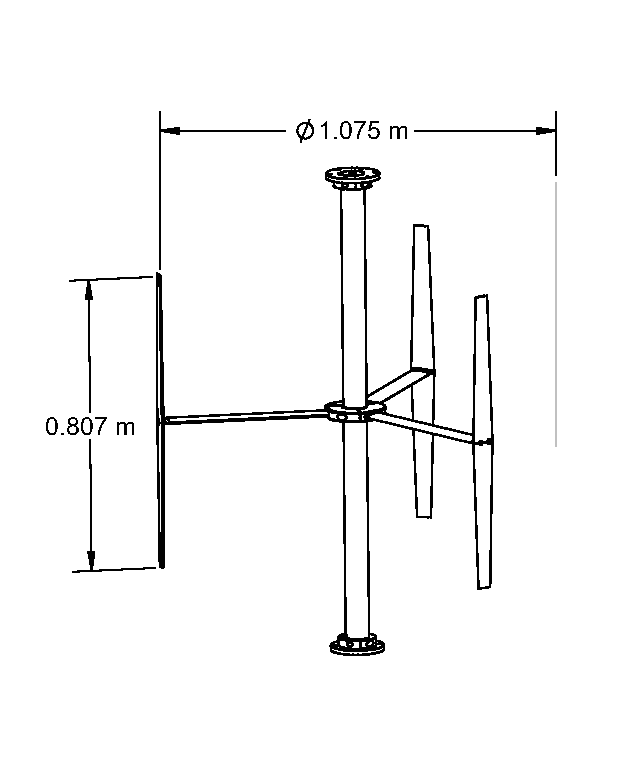
\includegraphics[width=0.65\textwidth]{figures/turbine.eps}

    \caption{{\bf Turbine Model.} A drawing of the turbine model.}

    \label{fig:turbine-drawing}
\end{figure}

For investigating the effects of support strut drag losses, a set of cylindrical
covers were designed to slip over the struts, which provided a significant
increase in strut drag. Endcaps were also fabricated to allow the high drag
strut cover configuration to be operated without blades. A drawing of the strut
covers is shown in Fig.~\ref{fig:covers}.

\begin{figure}[h]
    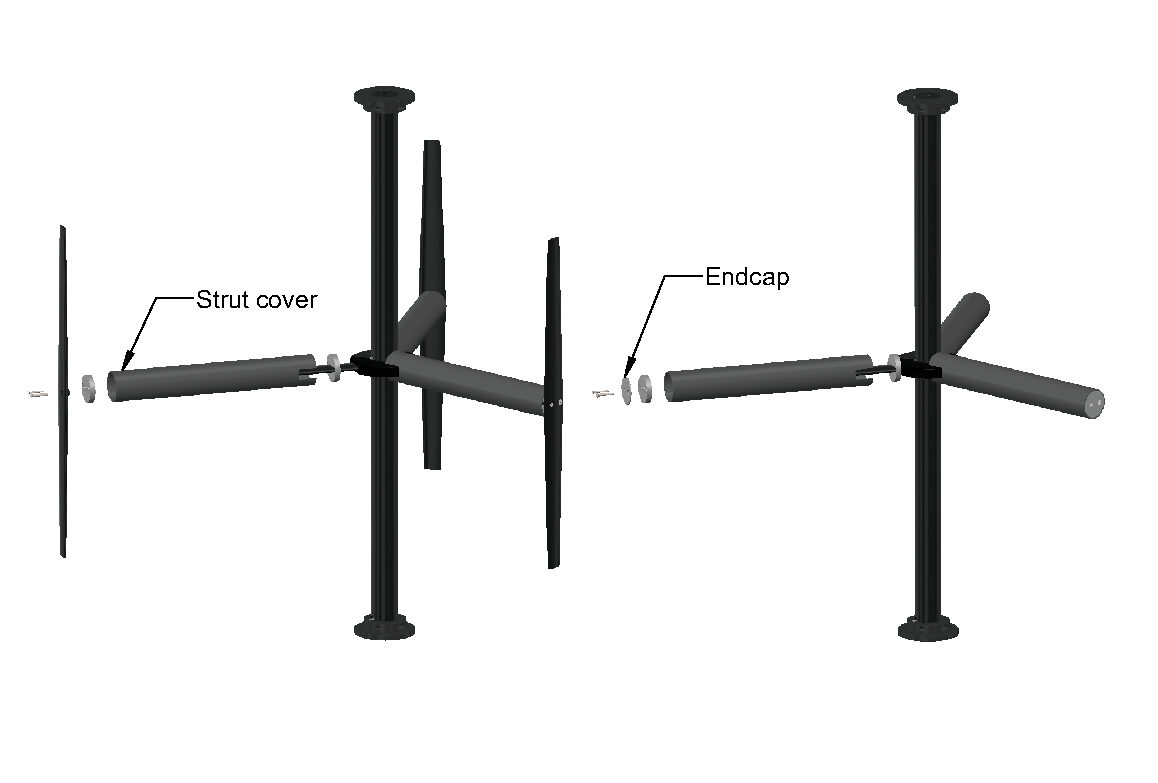
\includegraphics[width=0.95\textwidth]{figures/strut_covers.eps}
    
    \caption{{\bf Strut Covers.} A drawing of the high drag strut cover
        configuration with and without blades.}
    
    \label{fig:covers}
\end{figure}


\subsection*{Facility and instrumentation}

Experiments were performed in the UNH tow/wave tank, a 36 m long facility with a
3.66 m wide by 2.44 m deep cross-section, capable of tow speeds up to 3 m/s,
pictured in Fig.~\ref{fig:exp-setup}. The turbine was mounted in a frame built
from NACA 0020 struts, attached to the tow carriage by four linear bearings,
which transfer all streamwise force to a pair of S-beam load cells. The turbine
shaft RPM was controlled by a servo motor system, which allowed precise control
of the turbine tip speed ratio. The load torque was measured by an inline rotary
torque transducer. A load cell mounted at a fixed distance from the servo motor
via a moment arm provided a redundant torque measurement. Turbine shaft angle
was measured using the servo drive's emulated encoder output, set to $10^5$
counts per turbine shaft revolution. Carriage speed, and therefore inflow
velocity was measured using a linear encoder with 10 $\mu$m resolution. All of
these performance-related quantities were sampled at 2 kHz, while the tow tank's
motion controller provided redundant measurements of the carriage speed turbine
angular velocity sampled at 1 kHz. Turbine wake measurements at 1 meter
downstream were measured with a Nortek Vectrino+ acoustic Doppler velocimeter,
sampling at 200 Hz. A photo and drawing of the experimental setup are shown in
Fig.~\ref{fig:exp-setup-photo} and Fig.~\ref{fig:exp-setup}, respectively.


\begin{figure}[h]
    \centering

    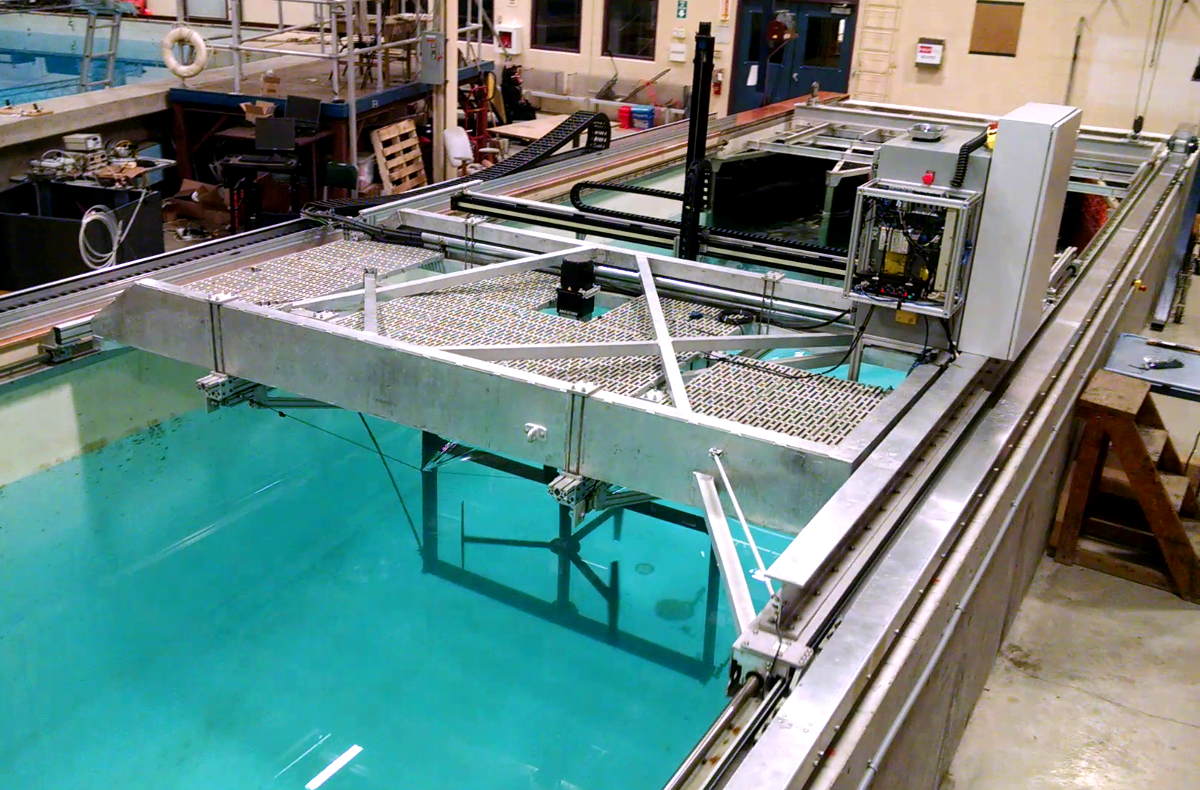
\includegraphics[width=0.95\textwidth]{figures/exp-setup-photo}

    \caption{\textbf{Experimental setup.} Photo of the UNH tow tank and turbine
    test bed with RM2 installed.}

    \label{fig:exp-setup-photo}
\end{figure}

\begin{figure}[h]
    \centering

    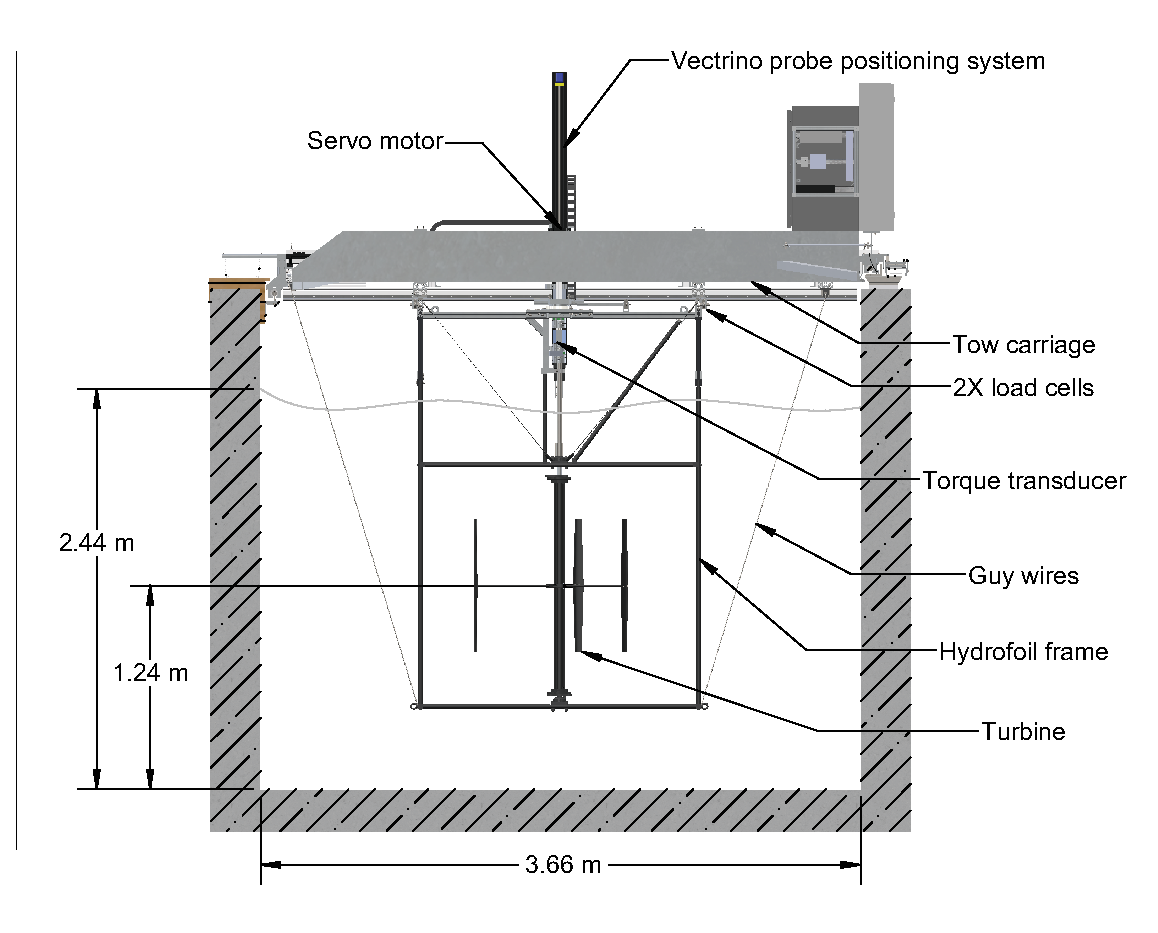
\includegraphics[clip,trim=0.01in 0 0 0,
    width=\textwidth]{figures/tank_cross_section}

    \caption{{\bf Experimental setup.} Illustration of the experimental setup.}

    \label{fig:exp-setup}
\end{figure}

\paragraph{Synchronization.} The three data acquisition instrumentation
subsystems---motion controller, NI DAQ (performance measurements), and Vectrino+
(wake velocity measurements)---started sampling at precisely the same time each
tow, after being triggered by a TTL pulse created by the motion controller. This
strategy retained synchronization for all performance signal samples (tow speed,
torque, drag, angular velocity), ensuring precise calculation of, e.g., power
coefficient. Since there is also synchronization of the initial sample from each
three subsystems, correlation of events in the performance and wake signals is
also possible.

\paragraph{Tare drag and torque compensation.} To best estimate the hydrodynamic
loads on the turbine rotor alone, tare torque and drag runs were performed to
measure the shaft bearing friction torque and turbine mounting frame drag,
respectively. Tare drag runs---measured with the turbine removed---were
performed for each tow speed in the experiment, for which the mean value was
subtracted in data processing, to arrive at an estimate for drag on the turbine
alone. Tare torque runs were performed by rotating the turbine shaft (without
blades) in air at constant angular velocity for a specified duration, over the
range of angular velocities used throughout the experiment. Tare torque was fit
with a linear regression versus shaft angular velocity, and added to the
measured turbine torque in post-processing.


\subsection*{Test parameters}

Data collection runs were separated into individual tows, for which all
independent variables---tow speed, tip speed ratio, velocity probe
position---were held constant. These runs were grouped into logical test matrix
``sections,'' in which typically a single independent variable was varied. Test
matrix section names and descriptions are provided in the \texttt{README.md}
file of the experimental data and code repository \cite{Bachant2015-RM2-data}.
Tow speed and their corresponding turbine diameter and blade chord Reynolds
numbers are presented in Tab.~\ref{tab:re}.

\begin{table}[ht]
\centering
\begin{tabular}{c|c|c|c|c}
Tow speed (m/s) & $Re_D$ & $Re_{c_\mathrm{tip}}$ & $Re_{c_\mathrm{root}}$ & $Re_{c_\mathrm{mid}}$\\
\hline
0.4 & $4.3 \times 10^5$ & $5.0 \times 10^4$ & $8.3 \times 10^4$ & $6.6 \times 10^4$ \\
0.6 & $6.5 \times 10^5$ & $7.4 \times 10^4$ & $1.2 \times 10^5$ & $9.9 \times 10^4$ \\
0.8 & $8.6 \times 10^5$ & $9.9 \times 10^4$ & $1.7 \times 10^5$ & $1.3 \times 10^5$ \\
1.0 & $1.1 \times 10^6$ & $1.2 \times 10^5$ & $2.1 \times 10^5$ & $1.7 \times 10^5$ \\
1.2 & $1.3 \times 10^6$ & $1.5 \times 10^5$ & $2.5 \times 10^5$ & $2.0 \times 10^5$ \\
\end{tabular}

\caption{{\bf Test Reynolds numbers.} Turbine diameter and approximate average
blade chord Reynolds numbers $Re_c \equiv \lambda U_\infty c / \nu$ at blade
tip, root, and mid-span, corresponding to various tow speeds at $\lambda=3.1$.}

\label{tab:re}
\end{table}

Wake measurements were all performed at 1 m downstream, which corresponds to
$x/D = 0.93$. The cross-stream and vertical coordinates are shown in
Fig.~\ref{fig:coordinates}.

\begin{figure}[h]
    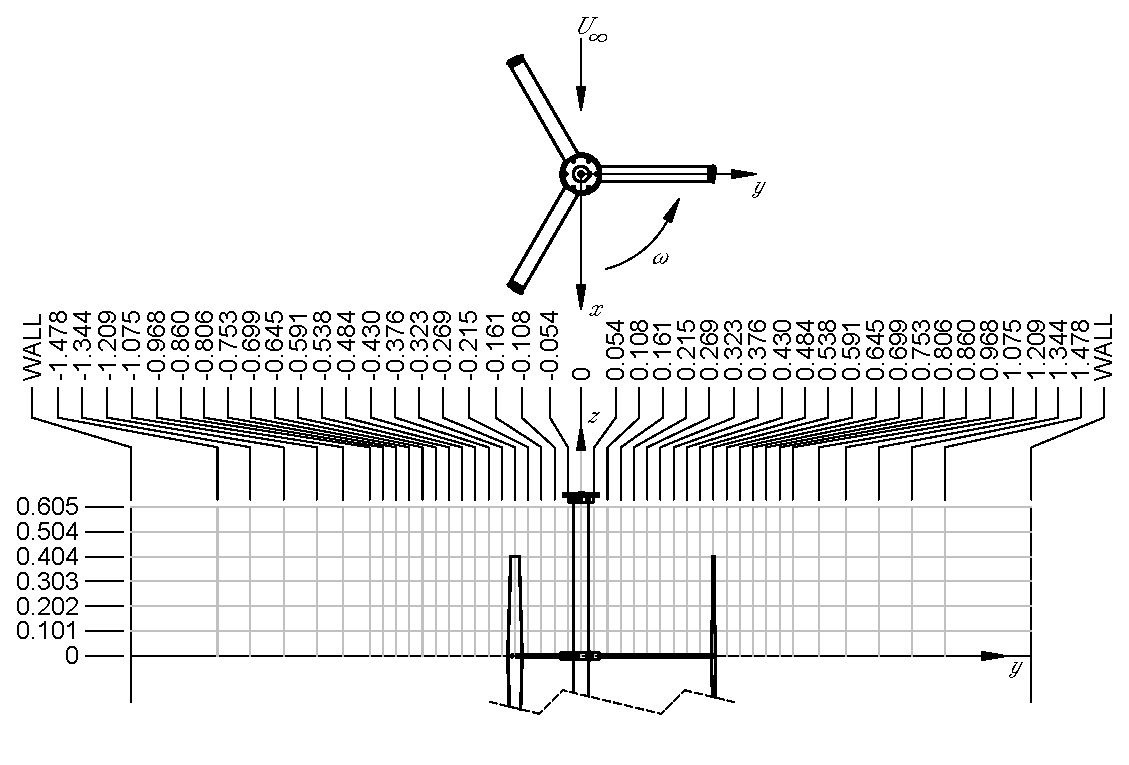
\includegraphics[width=\textwidth]{figures/turbine_coordinate_system.eps}

    \caption{{\bf Coordinate system.} Wake measurement coordinate system and
    cross-stream/vertical coordinates. All dimensions are in meters.}

    \label{fig:coordinates}
\end{figure}


\subsection*{Uncertainty Analysis}

Uncertainty was considered from a combination of systematic
and random errors. The random error was inferred from the sample standard
deviation and the systematic from the sensor calibrations or datasheets.
Combining both sources of error, along with their propagation into quantities
derived from multiple measurements, followed the procedures outlined in
Coleman and Steele (2009) \cite{ColemanSteele}, described below.

An expanded uncertainty interval with 95\% confidence was computed for
$\lambda$, $C_P$, and $C_D$
\begin{equation}
    U_{95} = t_{95} u_c,
\end{equation}
where $t_{95}$ is the value from the Student-$t$ distribution for a 95\%
confidence interval and $u_c$ is the combined standard uncertainty. Combined
standard uncertainty for a given quantity $X$ is calculated by
\begin{equation}
    u_X^2 = s_X^2 + b_X^2,
\end{equation}
where $s_X$ is the sample standard deviation, calculated as the standard
deviation of the mean per turbine revolution, and $b_X$ is the systematic
uncertainty, computed by
\begin{equation}
    b_{X}^2 = \sum_{i=1}^J \left( \frac{\partial X}{\partial x_i} \right)^2
    b_{x_i}^2,
\end{equation}
where $x_i$ is a primitive quantity used to calculate $X$ (e.g. $T$, $\omega$,
and $U_\infty$ for calculating $C_P$), and $b_{x_i}$ is the primitive quantity's
systematic uncertainty, estimated as half the value listed in
Table~\ref{tab-sensors}.

Selecting $t_{95}$ requires an estimate for degrees of freedom $\nu_X$, which
was obtained using the Welch--Satterthwaite formula
\begin{equation}
    \nu_X = \frac{\left(s_X^2 + \sum_{k=1}^M b_k^2 \right)^2} {s_X^4/\nu_{s_X} +
        \sum_{k=1}^M b_k^4/\nu_{b_k}},
\end{equation}
where $\nu_{s_X}$ is the number of degrees of freedom associated with $s_X$ and
$\nu_{b_k}$ is the number of degrees of freedom associated with $b_k$.
$\nu_{s_X}$ is assumed to be $(N-1)$, where $N$ is the number of independent
samples (or turbine revolutions). $\nu_{b_k}$ will be estimated as
\begin{equation}
    \nu_{b_k} = \frac{1}{2} \left( \frac{\Delta b_k}{b_k} \right)^{-2},
\end{equation}
where the quantity in parentheses is the relative uncertainty of $b_k$.

From previous measurements of a similarly-sized vertical-axis turbine with the
same experimental setup, we expect expanded uncertainties for $\lambda$, $C_P$,
and $C_D$ to be approximately 0.008, 0.01, and 0.02, respectively, at a tow
speed $U_\infty = 1.0$ m/s. These values are well within the discrepancies
between previous measurements and predictions by CACTUS \cite{Michelen2014},
making the data from the experiments described here suitable for model validation.


\subsection*{Data Processing}

For each tow speed, a relevant quasi-steady duration was selected by manually
inspecting a plot of the $C_P$ time series, and then truncated to include a
whole number of blade passages. Over this duration relevant statistics are
calculated.

To calculate turbine RPM from shaft angle, the encoder signal is differentiated
using a second order central difference scheme, after which a relatively
small-windowed moving average smoothing filter is applied to match the noise
level present in the redundant turbine RPM measurement from the motion
controller. A similar approach is used for calculating tow carriage speed
$U_\infty$ from carriage position measurements. Power and drag coefficients are
calculated as instantaneous quantities from the carriage speed as

\begin{equation}
    C_P = \frac{T \omega}{\frac{1}{2} \rho A U_\infty^3}
\end{equation}
and
\begin{equation}
    C_D = \frac{F_\mathrm{drag}}{\frac{1}{2} \rho A U_\infty^2},
\end{equation}
where $\rho$ is the fluid density (1000 kg/m\textsuperscript{3}) and $A$ is
the turbine frontal area $DH$.

All data processing and plotting code, along with the reduced dataset are
available from \cite{Bachant2015-RM2-data}. Note that this code will
automatically download raw data as necessary so users can perform a full
reanalysis of the measurements presented here.


\section*{Results and Discussion}

\subsection*{Performance}

Mean rotor power and drag coefficients for multiple Reynolds numbers are plotted
versus tip speed ratio in Fig.~\ref{fig:cp-curves} and Fig.~\ref{fig:cd-curves},
respectively. $C_P$ is shown to increase in general with $Re$, along with a
reduction in the optimal tip speed ratio, due to the tendency of foils to stall
at higher angles of attack at higher $Re$, and the higher angle of attack ranges
seen by the blades at lower $\lambda$. These effects diminish with increasing
$Re$, which is expected as the blade boundary layers transition to turbulence
closer to the leading edge \cite{Lissaman1983, Bachant2015-RVAT-Re-dep}.

Strict Reynolds number independence was not observed, i.e., the $C_P$ curves do
not collapse exactly onto each other. Note that the data collection was limited
at higher $Re$ and $\lambda$ due to the unsteady turbine force resonating with
the tow carriage drive belt. In contrast to the power coefficient data, the
rotor drag coefficient curves nearly collapse onto each other for $Re_D \ge 0.6
\times 10^6$.

\begin{figure}[h]
    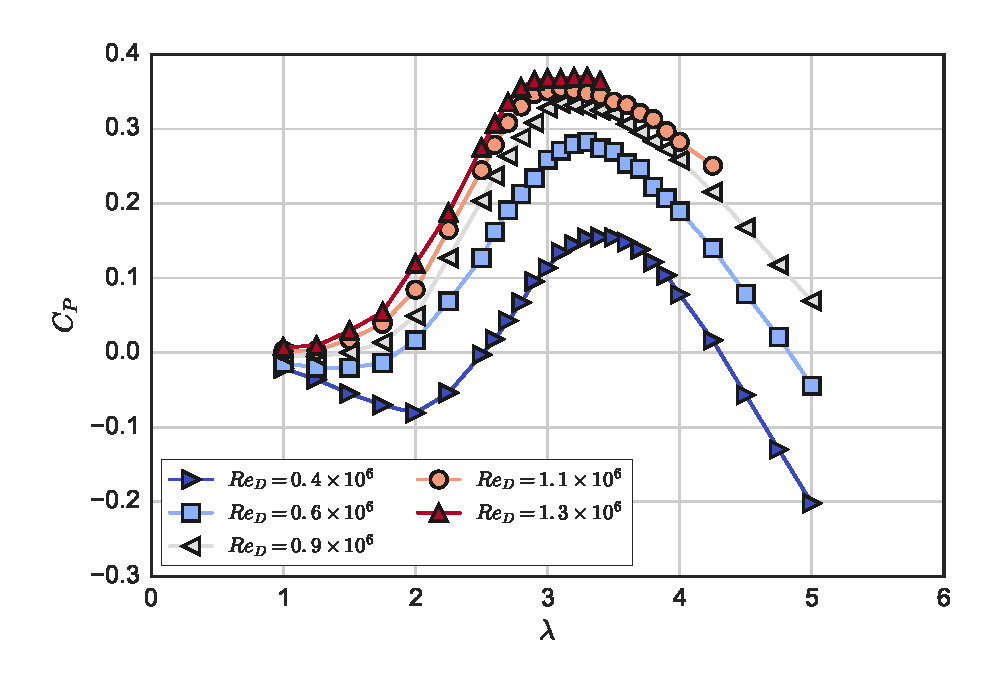
\includegraphics[width=\textwidth]{figures/cp_curves.eps}

    \caption{{\bf Power Coefficient Curves.} Mean rotor power coefficient
    plotted versus mean tip speed ratio for multiple Reynolds numbers.}

    \label{fig:cp-curves}
\end{figure}

\begin{figure}[h]
    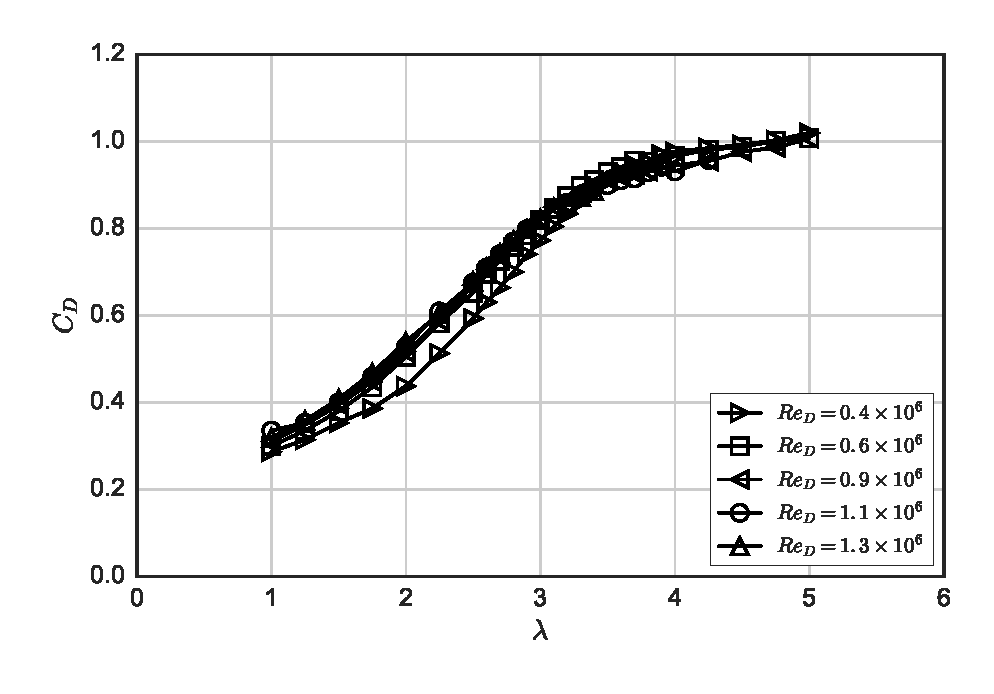
\includegraphics[width=\textwidth]{figures/cd_curves.eps}

    \caption{{\bf Drag Coefficient Curves.} Mean rotor drag coefficient plotted
    versus mean tip speed ratio for multiple Reynolds numbers.}

    \label{fig:cd-curves}
\end{figure}

The behavior of the power coefficient at $\lambda=3.1$ is plotted in
Fig.~\ref{fig:cp-re-dep}, where once again the increase in $C_P$ with $Re$ is
highlighted. We see that the power coefficient of the turbine increases
dramatically below $Re_D = 1 \times 10^6$ or $Re_c \equiv \lambda U_\infty c /
\nu \approx 2 \times 10^5$, beyond which there appears to be a small, linear,
positive trend. The tendency of $C_P$ to continue increasing slightly could be
an effect of lower virtual camber when compared to the strong $Re$-independence
of the higher $c/R$ UNH-RVAT \cite{Bachant2015-RVAT-Re-dep}.

\begin{figure}[h]
    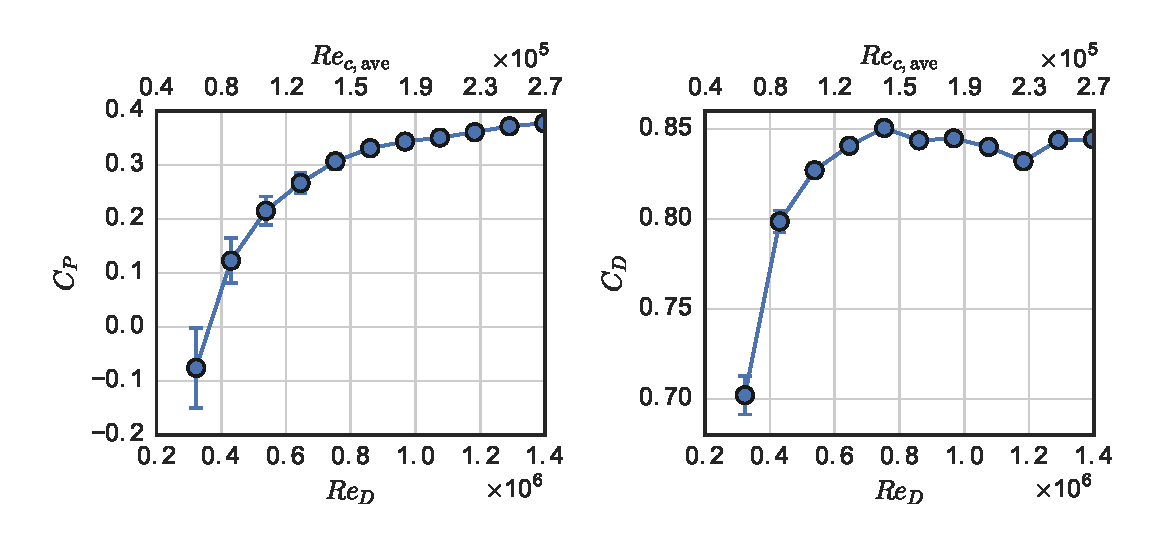
\includegraphics[width=\textwidth]{figures/perf_re_dep.eps}

    \caption{{\bf Reynolds Number effects on performance.} Power and drag
    coefficient at $\lambda=3.1$ plotted versus turbine diameter and approximate
    average blade root chord Reynolds number.}

    \label{fig:cp-re-dep}
\end{figure}


\subsection*{Wake characteristics}

The mean velocity field at a tip speed ratio $\lambda=3.1$, 1 m downstream
($x/D=0.93$) is plotted in Fig.~\ref{fig:meancontquiv}. The mean streamwise
velocity deficit is markedly more symmetric than that of the UNH-RVAT, with
lower acceleration around the turbine thanks to lower rotor drag coefficient and
blockage ratio \cite{Bachant2015-JoT}. We also see that the effects of blade tip
vortex shedding are relatively weaker, which is likely an effect of the RM2's
lower solidity and tapered blades.

\begin{figure}[h]
    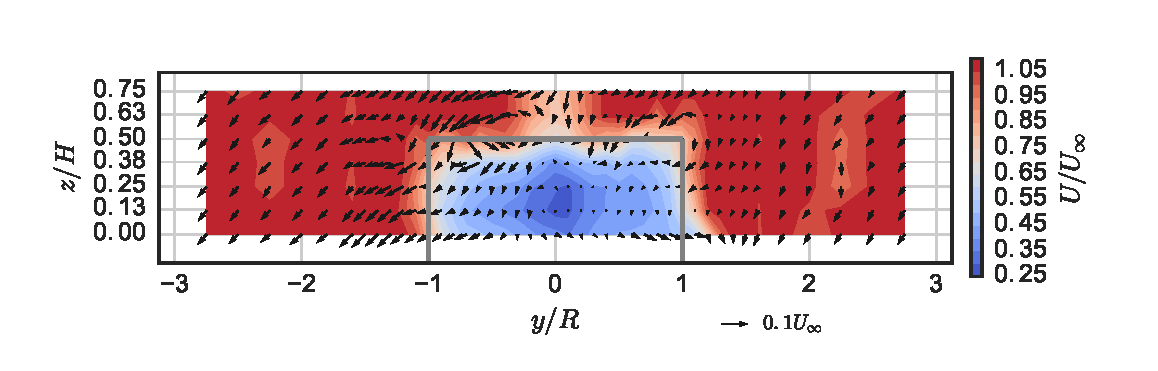
\includegraphics[width=\textwidth]{figures/meancontquiv.eps}

    \caption{{\bf Mean Velocity.} Mean velocity field (looking upstream) at 1 m
    downstream ($x/D=0.93$), $U_\infty=1.0$ m/s, and $\lambda=3.1$. Refer to
    Fig.~\ref{fig:coordinates} for turbine axis orientation. Solid dark gray
    lines indicate turbine frontal area.}

    \label{fig:meancontquiv}
\end{figure}


Fig.~\ref{fig:kcont} shows the turbulence kinetic energy in the turbine wake. We
mainly see unsteadiness in the flow generated by the blade tip vortex shedding
(the horizontal band around $z/H=0.5$). Compared with the UNH-RVAT, turbulence
generation is lower overall, without the intense vertical band around $y/R=-1$,
which indicates that the RM2 blades are operating further from
stall---consistent with the higher tip speed ratio operation.

\begin{figure}[h]
    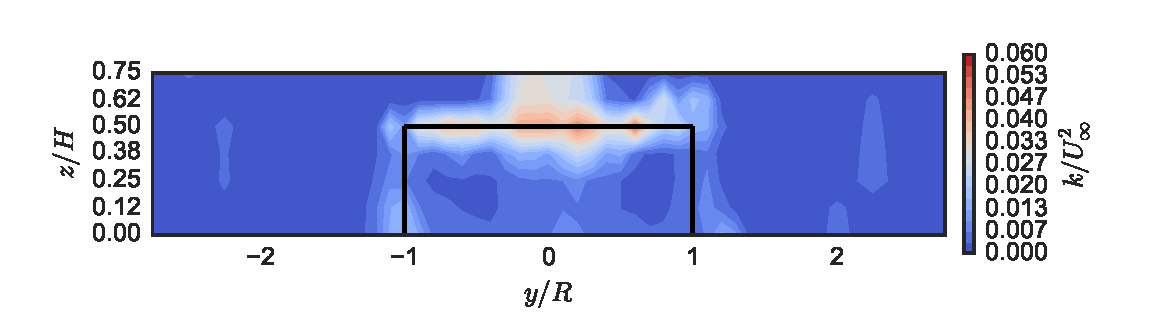
\includegraphics[width=\textwidth]{figures/k_contours.eps}

    \caption{{\bf Turbulence Kinetic Energy.} Turbulence kinetic energy (looking
    upstream) at 1 m downstream ($x/D=0.93$), $U_\infty=1.0$ m/s, and
    $\lambda=3.1$. Solid black lines indicate turbine frontal area.}

    \label{fig:kcont}
\end{figure}


Weighted averages for the transport terms in the mean kinetic energy
equation---analyzed identically to \cite{Bachant2015-JoT}---are shown in
Fig.~\ref{fig:Ktransport}. Due to the weaker blade vortex shedding, we see
transport due to vertical advection at this point in the wake is approximately 3
times lower than the higher solidity UNH-RVAT. Note that direct comparison is
somewhat invalid, since the total measurement plane area is about 5\% lower for
this experiment. However, the differences observed are beyond this discrepancy.
We also see relatively lower levels of cross-stream turbulent transport thanks
to the lack of blade stall vortex shedding. These results may have interesting
implications regarding the application of turbines with lower power coefficient
to possibly improve overall array performance through enhanced transport of
kinetic energy from the free stream, though a detailed anaylsis of the
downstream evolution and turbine interaction will be necessary.

\begin{figure}[ht!]
    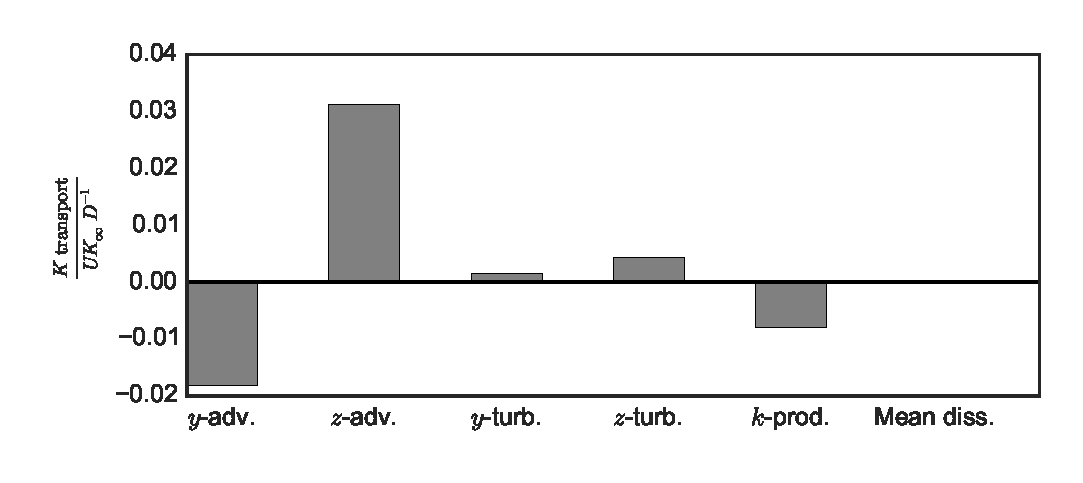
\includegraphics[width=0.9\textwidth]{figures/K_trans_bar_graph.eps}

    \caption{{\bf Mean Kinetic Energy Transport.} Weighted average estimates for
    terms contributing to streamwise recovery of mean kinetic energy, multiplied
    by two due to implied symmetry.}

    \label{fig:Ktransport}
\end{figure}


\subsection*{Strut drag losses}

Performance curves for the rotor with both NACA 0021 and cylindrical struts are
shown in Fig.~\ref{fig:perf-covers}. As expected, the high drag cylindrical
struts reduce performance dramatically, which worsens as $\lambda$ increases.
This is in accordance with the measurements of Rawlings \cite{Rawlings2008},
though the strut losses in this case are larger due to the very high drag profile.

\begin{figure}[ht!]
    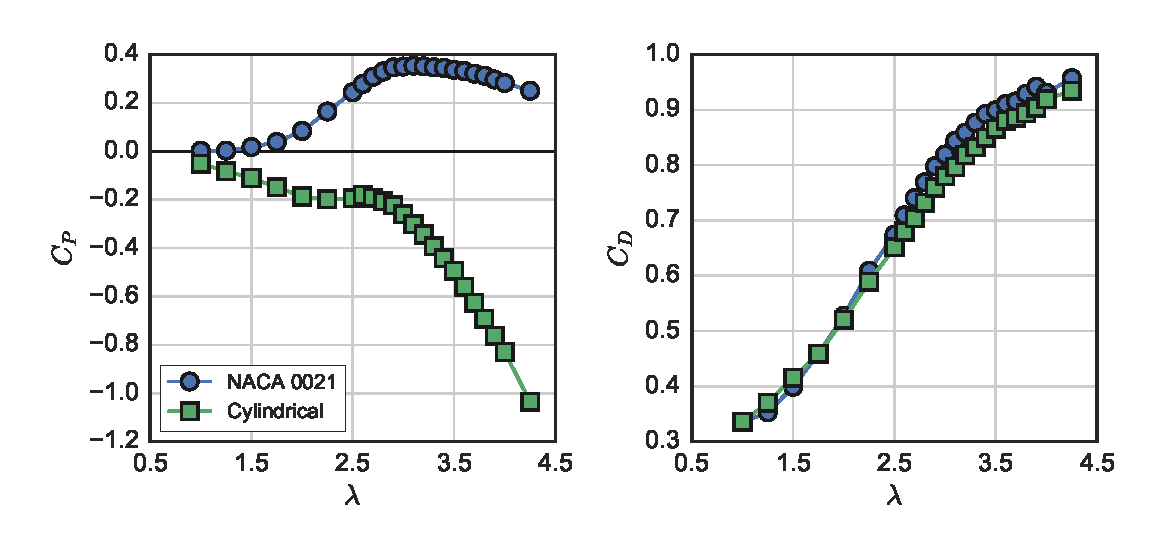
\includegraphics[width=\textwidth]{figures/perf_covers.eps}
    
    \caption{{\bf High drag strut performance.} Turbine performance and rotor
        drag coefficient curves with both NACA 0021 and cylindrical struts.}
    
    \label{fig:perf-covers}
\end{figure}

Measurements for the power coefficient contributions of the strut drag losses
are presented in Fig.~\ref{fig:no-blades} for NACA 0021 and cylindrical
struts---both in towed and stationary conditions. These are computed in the same
fashion as the curves in Fig.~\ref{fig:cp-curves}, but with the blades removed.
We see that strut drag losses increase with tip speed ratio to the power 2--3,
which makes streamlined struts much more important for low solidity turbines,
given the inverse correlation between solidity and $\lambda_0$
\cite{Templin1974}.

\begin{figure}[ht!]
    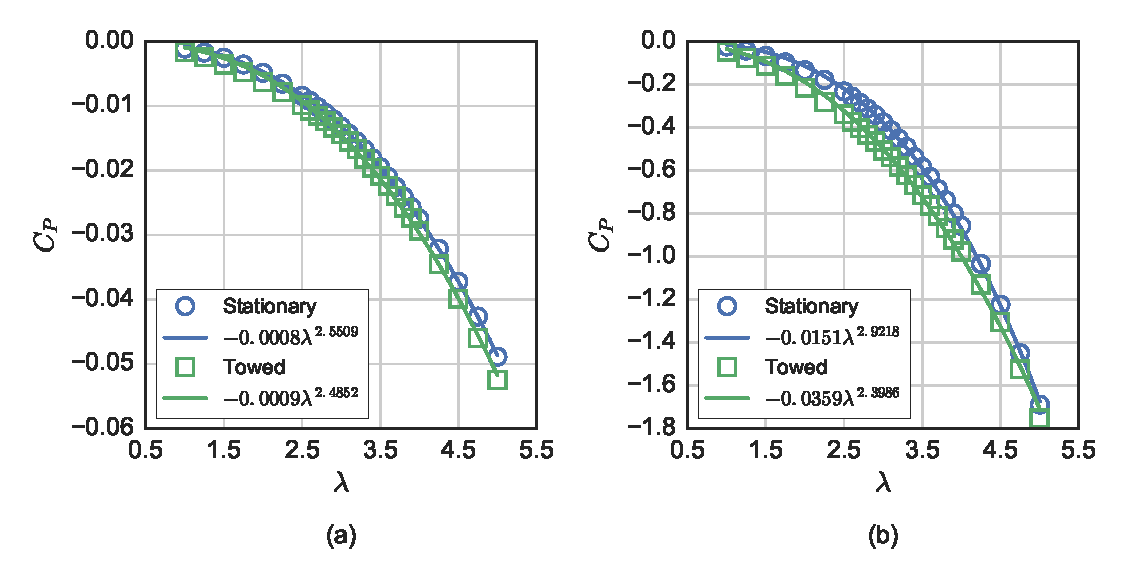
\includegraphics[width=\textwidth]{figures/no_blades_all.eps}

    \caption{{\bf Strut drag losses.} Measurements of the strut drag losses for
    (a) NACA 0021 and (b) cylindrical struts, both stationary and towed.}

    \label{fig:no-blades}
\end{figure}

Strut drag losses do not change much for the streamlined NACA 0021 struts in the
towed versus stationary configuration. However, for the cylindrical struts,
losses increase significantly when towed and operating in the mid range of tip
speed ratios. With respect to numerical modeling, these measurements will allow
support struts to be simulated without blades, to isolate and evaluate the
ability to predict these losses independent of the blade loading.


\subsection*{Conclusions}

The performance and near-wake for a 1:6 scale DOE Reference Model 2 cross-flow
turbine was measured in a towing tank. Performance was assessed for Reynolds
number dependence, showing a convergence to a weakly $Re$-dependent linear
regime at approximately $Re_D \approx 1 \times 10^6$ or $Re_{c,\mathrm{ave}}
\approx 2 \times 10^5$. Comparison was made between this turbine and the higher
solidity UNH-RVAT, tested in nearly identical conditions, which showed similar
Reynold number thresholds but a flatter linear regime, likely to due virtual
camber of the higher chord-to-radius ratio of the UNH-RVAT blades.

The wake at $x/D=0.93$ downstream was shown to be relatively symmetrical and
lacked the evidence of strong blade stall, which once again differentiates this
turbine from the UNH-RVAT. Terms from the mean kinetic energy transport equation
were also computed in this $y$--$z$ plane, showing the relative importance of
the vertical advection compared with turbulent transport terms at this location.
It is interesting to note that though the turbine is a more effective energy
converter than the UNH-RVAT, its wake recovery may in fact be slower due to
weaker blade tip vortex shedding.

The effects of parasitic drag from blade support struts on turbine performance
were measured by rotating the turbine without blades while stationary and while
towing. It is shown that these losses---even for a streamlined hydrofoil
strut---can become significant quickly at higher tip speed ratios---up to an
approximate 5 percentage point decrease in power coefficient at a tip speed
ratio of 5. These measurements were repeated with a set of high-drag cylindrical
struts, which as expected, prevented the turbine from producing any mechanical
power at any tip speed ratio. Nevertheless these measurements provide important
validation data for both high and low fidelity numerical performance prediction
models, allowing researchers to test models without blade effects.

This data, along with the code for processing and visualization, is provided
openly via a Creative Commons license, and is available from
\cite{Bachant2015-RM2-data}. The authors hope that this can provide
opportunities for extensive validation of predictive tools for the complex
unsteady flow physics of cross-flow turbines.


\section*{Acknowledgments}

This study was supported by the Department of Energy (DOE), Office of Energy
Efficiency and Renewable Energy (EERE), Wind and Water Power Technologies Office
(WWPTO). Sandia National Laboratories is a multi-program laboratory managed and
operated by Sandia Corporation, a wholly owned subsidiary of Lockheed Martin
Corporation, for the U.S. Department of Energy's National Nuclear Security
Administration under contract DE-AC04-94AL85000.

\nolinenumbers

% Compile your BiBTeX database using our plos2015.bst
% style file and paste the contents of your .bbl file
% here.
%
\bibliographystyle{plos2015}
\bibliography{library}


\end{document}
